\documentclass[10pt,landscape,a4paper]{article}
\usepackage[utf8]{inputenc}
\usepackage[ngerman]{babel}
\usepackage{tikz}
\usetikzlibrary{shapes,positioning,arrows,fit,calc,graphs,graphs.standard}
\usepackage[nosf]{kpfonts}
\usepackage[t1]{sourcesanspro}
%\usepackage[lf]{MyriadPro}
%\usepackage[lf,minionint]{MinionPro}
\usepackage{multicol}
\usepackage{wrapfig}
\usepackage[top=0mm,bottom=1mm,left=0mm,right=1mm]{geometry}
\usepackage[framemethod=tikz]{mdframed}
\usepackage{microtype}
\usepackage{amsmath}

\let\bar\overline

\definecolor{myblue}{cmyk}{1,.72,0,.38}
\definecolor{forestgreen}{RGB}{34,139,34}

\def\firstcircle{(0,0) circle (1.5cm)}
\def\secondcircle{(0:2cm) circle (1.5cm)}

\colorlet{circle edge}{myblue}
\colorlet{circle area}{myblue!5}

\tikzset{filled/.style={fill=circle area, draw=circle edge, thick},
    outline/.style={draw=circle edge, thick}}

\pgfdeclarelayer{background}
\pgfsetlayers{background,main}

\everymath\expandafter{\the\everymath \color{myblue}}
\everydisplay\expandafter{\the\everydisplay \color{myblue}}

\renewcommand{\baselinestretch}{.8}
\pagestyle{empty}

\global\mdfdefinestyle{header}{%
linecolor=gray,linewidth=1pt,%
leftmargin=0mm,rightmargin=0mm,skipbelow=0mm,skipabove=0mm,
}

\newcommand{\header}{
\begin{mdframed}[style=header]
\footnotesize
\sffamily
Cryptography\\
by~Wei~Wu,~page~\thepage~of~2
\end{mdframed}
}

\makeatletter
\renewcommand{\section}{\@startsection{section}{1}{0mm}%
                                {.2ex}%
                                {.2ex}%x
                                {\color{myblue}\sffamily\small\bfseries}}
\renewcommand{\subsection}{\@startsection{subsection}{1}{0mm}%
                                {.2ex}%
                                {.2ex}%x
                                {\sffamily\bfseries}}



\def\multi@column@out{%
   \ifnum\outputpenalty <-\@M
   \speci@ls \else
   \ifvoid\colbreak@box\else
     \mult@info\@ne{Re-adding forced
               break(s) for splitting}%
     \setbox\@cclv\vbox{%
        \unvbox\colbreak@box
        \penalty-\@Mv\unvbox\@cclv}%
   \fi
   \splittopskip\topskip
   \splitmaxdepth\maxdepth
   \dimen@\@colroom
   \divide\skip\footins\col@number
   \ifvoid\footins \else
      \leave@mult@footins
   \fi
   \let\ifshr@kingsaved\ifshr@king
   \ifvbox \@kludgeins
     \advance \dimen@ -\ht\@kludgeins
     \ifdim \wd\@kludgeins>\z@
        \shr@nkingtrue
     \fi
   \fi
   \process@cols\mult@gfirstbox{%
%%%%% START CHANGE
\ifnum\count@=\numexpr\mult@rightbox+2\relax
          \setbox\count@\vsplit\@cclv to \dimexpr \dimen@-1cm\relax
\setbox\count@\vbox to \dimen@{\vbox to 1cm{\header}\unvbox\count@\vss}%
\else
      \setbox\count@\vsplit\@cclv to \dimen@
\fi
%%%%% END CHANGE
            \set@keptmarks
            \setbox\count@
                 \vbox to\dimen@
                  {\unvbox\count@
                   \remove@discardable@items
                   \ifshr@nking\vfill\fi}%
           }%
   \setbox\mult@rightbox
       \vsplit\@cclv to\dimen@
   \set@keptmarks
   \setbox\mult@rightbox\vbox to\dimen@
          {\unvbox\mult@rightbox
           \remove@discardable@items
           \ifshr@nking\vfill\fi}%
   \let\ifshr@king\ifshr@kingsaved
   \ifvoid\@cclv \else
       \unvbox\@cclv
       \ifnum\outputpenalty=\@M
       \else
          \penalty\outputpenalty
       \fi
       \ifvoid\footins\else
         \PackageWarning{multicol}%
          {I moved some lines to
           the next page.\MessageBreak
           Footnotes on page
           \thepage\space might be wrong}%
       \fi
       \ifnum \c@tracingmulticols>\thr@@
                    \hrule\allowbreak \fi
   \fi
   \ifx\@empty\kept@firstmark
      \let\firstmark\kept@topmark
      \let\botmark\kept@topmark
   \else
      \let\firstmark\kept@firstmark
      \let\botmark\kept@botmark
   \fi
   \let\topmark\kept@topmark
   \mult@info\tw@
        {Use kept top mark:\MessageBreak
          \meaning\kept@topmark
         \MessageBreak
         Use kept first mark:\MessageBreak
          \meaning\kept@firstmark
        \MessageBreak
         Use kept bot mark:\MessageBreak
          \meaning\kept@botmark
        \MessageBreak
         Produce first mark:\MessageBreak
          \meaning\firstmark
        \MessageBreak
        Produce bot mark:\MessageBreak
          \meaning\botmark
         \@gobbletwo}%
   \setbox\@cclv\vbox{\unvbox\partial@page
                      \page@sofar}%
   \@makecol\@outputpage
     \global\let\kept@topmark\botmark
     \global\let\kept@firstmark\@empty
     \global\let\kept@botmark\@empty
     \mult@info\tw@
        {(Re)Init top mark:\MessageBreak
         \meaning\kept@topmark
         \@gobbletwo}%
   \global\@colroom\@colht
   \global \@mparbottom \z@
   \process@deferreds
   \@whilesw\if@fcolmade\fi{\@outputpage
      \global\@colroom\@colht
      \process@deferreds}%
   \mult@info\@ne
     {Colroom:\MessageBreak
      \the\@colht\space
              after float space removed
              = \the\@colroom \@gobble}%
    \set@mult@vsize \global
  \fi}

\makeatother
\setlength{\parindent}{0pt}

\begin{document}
\small
\begin{multicols*}{5}
	\section{Mathematical Basic}
\subsection*{Identities and Inequalities}
Binomial expansion theorem:\\
$(x+y)^n=\sum_{i=0}^{n}\binom{n}{i}x^i y^{n-i}$\\
Proposition:\\
\begin{itemize}
    \item For all $x\ge 1$ it holds that $(1-1/x)^x\le e^{-1}$
    \item For all $x$ it holds that $1-x\le e^{-x}$
    \item For all $x$ with $0\le x \le 1$ it holds that
\end{itemize}
$e^{-x}\le 1-(1-\frac{1}{e})\cdot x\le 1-\frac{x}{2}$\\
\subsection*{Asymptotic Notation}
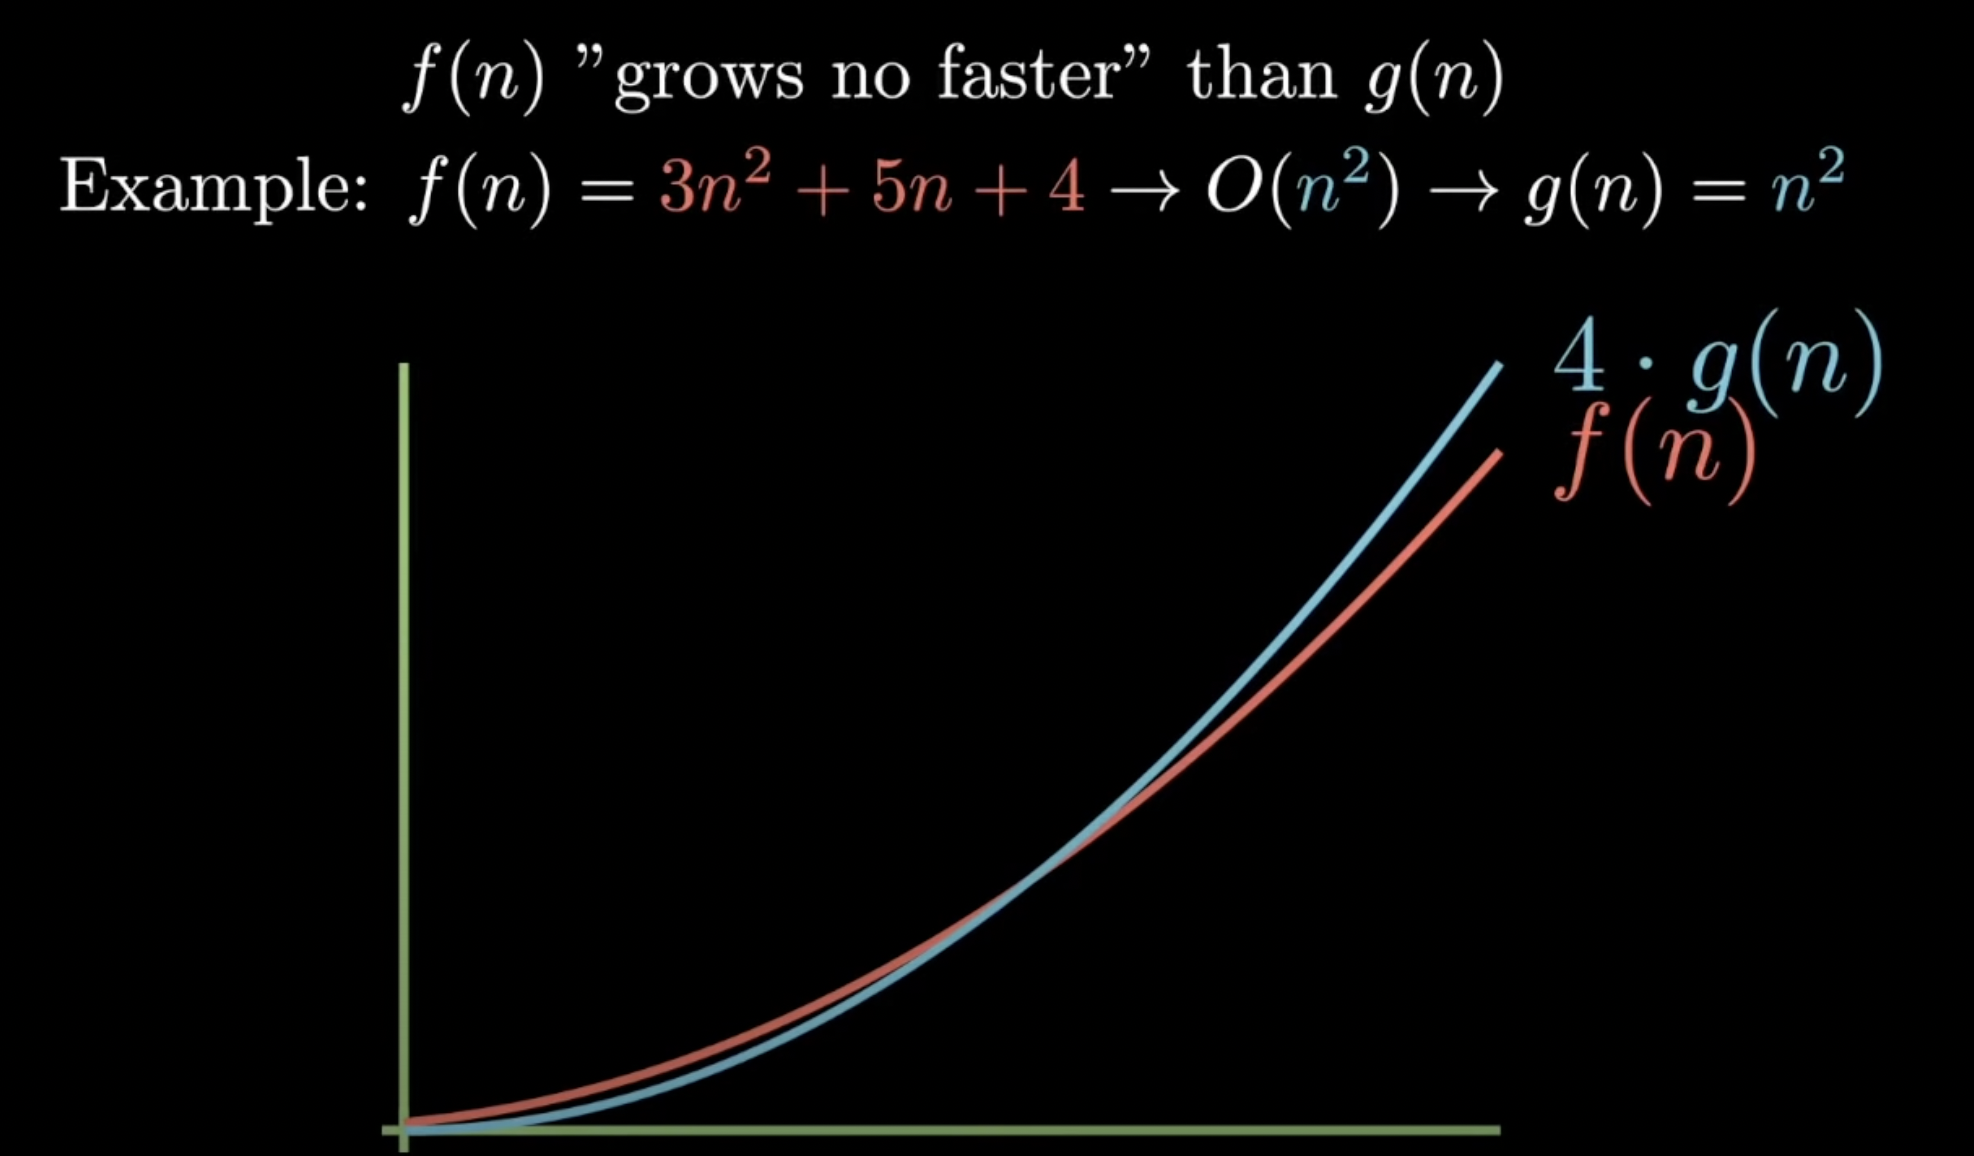
\includegraphics[width=\columnwidth]{big-o-explained.png}
Let $f(n),g(n)$ be functions from non-negative integers to non-negative reals. 
Then:
\begin{itemize}
    \item $f(n)=\mathcal{O}(g(n))$ means that there exist positive integers c 
    and n' such that for all $n > n'$ it holds that $f(n)\le c \cdot g(n)$
    \item $f(n)=\varOmega (g(n))$ means that there exist positive integers c
    and n' such that for all $n > n'$ it holds that $f(n)\ge c\cdot g(n)$.
    \item $f(n)=\varTheta (g(n))$ means that there exist positive integers 
    $c_{1}$ and $c_{2}$ such that for all $n > n'$ it holds that 
    $c_{1}\cdot g(n) \le f(n) \le c_{2} \cdot g(n)$
    \item $f(n)=o(g(n))$ means that $\lim_{n \to \infty} \frac{f(n)}{g(n)}=0$ 
    \item $f(n)=\omega (g(n))$ means that 
    $\lim_{n \to \infty} \frac{f(n)}{g(n)}=\infty$ 
\end{itemize}

\subsection*{Basic Probability}

By definition:\\
$\Pr[E] = 1 - \Pr[\bar{E}]$\\
$\Pr[E_1\wedge E_2]\le \Pr[E_1]$\\
$\Pr[E_1 \vee E_2]\ge\Pr[E_1]$\\
When $E_1$ $E_2$ are independent:\\
$\Pr[E_1\wedge E_2]=\Pr[E_1] \cdot \Pr[E_2]$\\
Union Bound:\\
$\Pr[E_1\vee E_2]\le\Pr[E_1]+\Pr[E_2]$\\
Bayes' Theorem:\\
$\Pr[E_1|E_2] = \frac{\Pr[E_2|E_1]\cdot\Pr[E_1]}{\Pr[E_2]}$\\
Let $E_1,\cdots ,E_n$ be events such that $Pr[E_1\vee\cdots E_n]=1$ and 
$\Pr[E_i\wedge E_j]=0$ for all $i\neq j$. That is, the ${E_i}$ \emph{partition} 
the space of all possible events, so that with probability 1 exactly one of the
events $E_i$ occurs. Then for any F:\\
$\Pr[F]=\sum_{i=1}^{n}\Pr[F\wedge E_i]$\\
when $n=2$ and $E_2=\bar{E}_1$, giving:\\
$\Pr[F]=\Pr[F|E_1]\cdot\Pr[E_1]+\Pr[F|\bar{E}_1]\cdot\Pr[\bar{E}_1]$\\
we get a tighter union bound:\\
$\Pr[E_1\vee E_2]\le\Pr[E_1]+\Pr[E_2|\bar{E}_1]$\\
$\Pr[\vee^{k}_{i=1}E_{i}]
\le\Pr[E_1]+\sum^{k}_{i=2}\Pr[E_i|\bar{E}_1\wedge\cdots\wedge\bar{E}_{i-1}]$\\
   \section{Introduction}
Definition of security's components:
\begin{enumerate}
    \item threat model
    \item security goal
\end{enumerate}

Adversary types:
\begin{itemize}
    \item Known-plaintext attack:\\
    $\{x_i,F_k(x_i)\}$ with $x_i$ known to $\mathcal{A}$
    \item Chosen-plaintext attack:\\
    $\{F_k(x_i)\}$ for $x_i$ chosen by $\mathcal{A}$
    \item Chosen-ciphertext attack:\\
    $\{F_k(x_i)\},\{F_k^{-1}(y_i)\}$ for $x_i$,$y_i$ chosen by $\mathcal{A}$
\end{itemize}
   \section{Perfectly Secret Encryption}

\subsection*{Definition}
key: $k \in \mathcal{K}$ The distribution over $\mathcal{K}$ is 
the one defined by running $Gen$ and taking the output.\\
message: $m \in \mathcal{M}$\\
$c\leftarrow Enc_k(m)$: 
possibly probabilistic process by which 
message m is encrypted using key $k$ to give ciphertext $c$\\
$x \leftarrow S$: uniform selection of $x$ from a set $S$\\
$\mathcal{C}$: set of all possible ciphertexts 
that can be output by $Enc_k(m)$\\\\
let $K$ be a random variable denoting the value of the key output by $Gen$:
for any $k \in \mathcal{K},\ \Pr[K=k]$ denotes the probability that key output
by $Gen$ is equal to $k$\\\\
let $M$ be a random variable denoting the message being encrypted:
$\Pr[M=m]$ denotes the probability that the message takes on the value
$m \in \mathcal{M}$\\\\
$\ast\ $The probability distribution of the message is not 
determined by the encryption scheme itself, but instead reflects the likelihood
 of different messages being sent by the parties using the scheme, as well as an
 adversary’s uncertainty about what will be sent.\\
 $\ast\ $ $K$ and $M$ are assumed to be independent.\\\\
 Fixing an encryption scheme and a distribution over $\mathcal{M}$ determines a
 distribution over the space of ciphertexts $\mathcal{C}$ given by choosing
  a key $k \in \mathcal{K}$ and a message $m \in \mathcal{M}$, and then 
  computing the ciphertext $c \leftarrow Enc_k(m)$. Let $C$ be the random 
  variable denoting the resulting ciphertext and so, for $c \in \mathcal{C}$,
  $\Pr[C=c]$ denote the probability that the ciphertext is equal to the 
  fixed value $c$

\subsection*{Perfect secrecy} 
ciphertext should have \emph{no effect} on the adversary’s 
knowledge regarding the actual message that was sent\\
Definition: \emph{An encryption scheme 
\emph{(Gen,Enc,Dec)} with message space $\mathcal{M}$ is perfectly secret 
if for every probability distribution over $\mathcal{M}$, 
every message $m \in \mathcal{M}$, and every 
ciphertext $c \in \mathcal{C}$ for which $\Pr[C = c] > 0$:}
$\Pr[M=m|C=c]=Pr[M=m]$\\
   \section{Private-Key Encryption}
\subsection*{Computational Security}
Concrete approach:
\begin{enumerate}
    \item Security is only guaranteed against \emph{efficient} 
    adversaries that run for some feasible amount of time
    \item Adversaries can potentially succeed
     with some \emph{very small probability}
\end{enumerate}

A scheme is $(t,\varepsilon)-secure$ if any adversary running for time at most
 $t$ succeeds in breaking the scheme with probability at most $\varepsilon$.\\

 Asymptotic approach:\\
view the running time of the adversary, as well as its success probability, 
 as functions of the security parameter rather than as concrete numbers:
 \begin{enumerate}
     \item We equate “efficient adversaries” with randomized 
     algorithms running in time polynomial in n.
     \item We equate the notion of “small probabilities of success” 
     with success probabilities smaller than any inverse polynomial in n
 \end{enumerate}
 $PPT$: probabilistic polynomial-time\\
 Asymptotic security: A scheme is \emph{secure} if any ppt adversary succeeds
  in breaking the scheme with at most negligible probability.\\

  DEFINITION 3.7: A \emph{private-key encryption scheme} is a tuple of 
  probabilistic polynomial-time algorithms $(Gen, Enc, Dec)$ such that:
  \begin{enumerate}
      \item The \emph{key-generation algorithm Gen} takes as input $1^n$ and outputs
       a key $k$; we write $k \leftarrow Gen(1^n)$(emphasizing that Gen 
       is a randomized algorithm). We assume w.l.o.g that any
        key $k$ output by $Gen(1^n)$ satisfies $|k| \ge n$.
        \item The \emph{encryption algorithm Enc} takes as input a key $k$ and a plaintext
        message $m \in \{0,1\}\ast$, and outputs a ciphertext $c$. Since $Enc$
        may be randomized, we write this as $c \leftarrow Enc_k(m)$.
        \item The \emph{decryption algorithm Dec} takes as input a key $k$ and a ciphertext
        $c$, and outputs a message $m$ or an error. We assume that $Dec$ is 
        deterministic, and so write $m := Dec_k(c)$ 
        (assuming here that Dec does not return an error). 
        We denote a generic error by the symbol $\bot $.
  \end{enumerate}

It is required that for every $n$, every key $k$ output by $Gen(1^n)$, 
and every $m \in \{0,1\}\ast$, it holds that $Dec_k(Enc_k(m)) = m$.\\

$PrivK^{eav}_{\mathcal{A},\Pi}(n)$: 
\begin{enumerate}
    \item The adversary $\mathcal{A}$ is given input $1^n$, and outputs a
     pair of messages $m_0$, $m_1$ with $|m_0| = |m_1|$.
    \item A key $k$ is generated by running $Gen(1^n)$, and a uniform bit
     $b \in \{0,1\}$ is chosen. Ciphertext $c \leftarrow Enc_k(mb)$ is computed
      and given to $\mathcal{A}$. We refer to $c$ as the challenge ciphertext.
    \item $\mathcal{A}$ outputs a bit $b'$
    \item The output of the experiment is defined to be 1 if $b'=b$, and 0
    otherwise.
\end{enumerate}

DEFINITION 3.8: A private-key encryption scheme $\Pi = (Gen, Enc, Dec)$
 has \emph{indistinguishable encryptions in the presence of an eavesdropper}, or 
 is \emph{EAV-secure}, if for all probabilistic polynomial-time adversaries $\mathcal{A}$
 there is a negligible function \emph{negl} such that, for all $n$,
 $\Pr[PrivK^{eav}_{\mathcal{A},\Pi}(n)=1]\le\frac{1}{2}+negl(n)$\\

DEFINITION 3.9: A private-key encryption scheme $\Pi = (Gen, Enc, Dec)$
has \emph{indistinguishable encryptions in the presence of an eavesdropper}
if for all ppt adversaries $\mathcal{A}$ there is a negligible function $negl$ such that
$\Pr[out_{\mathcal{A}}(PrivK^{eav}_{\mathcal{A},\Pi}(n,0)=1)]
-\Pr[out_{\mathcal{A}}(PrivK^{eav}_{\mathcal{A},\Pi}(n,1)=1)]
\le negl(n)$\\
$\ast\ $Essentially states that no $\mathcal{A}$ can determine whether it is running in
experiment 0 or experiment 1\\

DEFINITION 3.14 (PRG): Let $\ell$ be a polynomial and let $G$ be a deterministic 
polynomial-time algorithm such that for any $n$ and any input $s \in \{0,1\}^n$, 
the result $G(s)$ is a string of length $\ell(n)$. We say that $G$ is 
a \emph{pseudorandom generator} if the following conditions hold:
\begin{enumerate}
    \item (Expainsion:) For every n it holds that $\ell(n)>n$
    \item (Pseudorandomness:) For any PPT algorithm $D$, there is a negligible
     function $negl$ such that $|\Pr[D(G(s))=1]-\Pr[D(r)=1]|\le negl(n)$,
     where the first probability is taken over uniform choice of
     $s \in \{0, 1\}^n$ and the randomness of $D$, and the second probability
      is taken over uniform choice of $r \in \{0, 1\}^{\ell(n)}$ and the randomness
       of $D$. We call $\ell$ the expansion factor of $G$
\end{enumerate}
Let $G:\{0,1\}^n\rightarrow \{0,1\}^{\ell(n)}$ be a deterministic poly-time
algorithm.\\
$PRG_{\mathcal{D},G}(n)$:
\begin{enumerate}
  \item The challenger chooses $b\leftarrow\{0,1\}$.\\
  if $b=0$, he chooses $r\leftarrow\{0,1\}^{\ell(n)}$\\
  if $b=1$, he chooses $s\leftarrow\{0,1\}^n$, and computes $r=G(s)$\\
  He gives $r$ to $\mathcal{D}$
  \item On input $r$, the distinguisher $\mathcal{D}$ outputs a guess $b'$
  \item $PRG_{\mathcal{D},G}(n)=1$, if $b'=b$
\end{enumerate}

Proofs by Reduction: We begin with an assumption that some problem $X$
 cannot be solved (in some precisely defined sense) by any polynomial-time
  algorithm, except with negligible probability. We want to prove that some
   cryptographic construction $\Pi$ is secure (again, in some sense that is 
   precisely defined).
   \begin{enumerate}
       \item Fix some efficient (i.e., probabilistic polynomial-time)
        adversary $\mathcal{A}$ attacking $\Pi$. Denote this adversary’s
         success probability by $\varepsilon(n)$.
       \item Construct an efficient algorithm $\mathcal{A}'$, called the “reduction,” 
       that attempts to solve problem $X$ using adversary $\mathcal{A}$ as a 
       subroutine. An important point here is that $\mathcal{A}'$ knows nothing
        about how $\mathcal{A}$ works; the only thing $\mathcal{A}'$ knows 
        is that $\mathcal{A}$ is expecting to attack $\Pi$. So, given some input
         instance $x$ of problem $X$, our algorithm $\mathcal{A}'$ will simulate
          for $\mathcal{A}$ an instance of $\Pi$ such that:
          \begin{enumerate}
              \item As far as $\mathcal{A}$ can tell, it is interacting with 
              $\Pi$. That is, the view of $\mathcal{A}$ when run as a subroutine
               by $\mathcal{A}'$ should be distributed identically to 
               (or at least close to) the view of $\mathcal{A}$ when it
                interacts with $\Pi$ itself.
              \item If $\mathcal{A}$ succeeds in “breaking” the instance of 
              $\Pi$ that is being simulated by $\mathcal{A}'$, this should 
              allow $\mathcal{A}'$ to solve the instance $x$ it was given, 
              at least with inverse polynomial probability $1/p(n)$.
          \end{enumerate}
        \item Taken together, 2(a) and 2(b) imply that $\mathcal{A}'$ solves $X$
         with probability $\varepsilon(n)/p(n)$. If $\varepsilon(n)$ is not 
         negligible, then neither is $\varepsilon(n)/p(n)$. Moreover, 
         if $\mathcal{A}$ is efficient then we obtain an efficient algorithm 
         $\mathcal{A}'$ solving $X$ with non-negligible probability, 
         contradicting the initial assumption.
        \item Given our assumption regarding $X$, we conclude that no efficient 
        adversary $\mathcal{A}$ can succeed in breaking $\Pi$ with 
        non-negligible probability. Stated differently, 
        $\Pi$ is computationally secure.
   \end{enumerate}
CPA Security:
\begin{enumerate}
  \item $\mathcal{A}$ is allowed to request encryptions (under key $k$) of any messages of its choice.
  \item $\mathcal{A}$ still cannot learn any information about encrypted message when seeing challenge ciphertext $c$.
\end{enumerate}
Oracle: An oracle evaluates a function without revealing its internal details.
We write $\mathcal{A}^{O(\cdot)}$ to indicate a party 
$\mathcal{A}$ given oracle access to some function $O$.
$PrivK^{cpa}_{\mathcal{A},\Pi}(n)$:
\begin{enumerate}
  \item The challenger chooses $k\leftarrow Gen(1^n)$
  \item $\mathcal{A}^{Enc_k(\cdot)}(1^n)$ outputs $m_0, m_1$ such that
  $|m_0|=|m_1|$
  \item The challenger chooses $b\leftarrow\{0,1\}$, 
  computes $c \leftarrow Enc_k(m_b)$ and gives $c$ to $\mathcal{A}$
  \item $\mathcal{A}^{Enc_k(\cdot)}$ outputs guess bit $b'$
\end{enumerate}
$PRF_{\mathcal{D},F}(n)$:
\begin{enumerate}
  \item The challenger chooses $b \in \{0,1\}$.
  \item If $b=0$,he chooses $f \leftarrow F_n$ and 
  gives $\mathcal{D}$ an oracle$ O=f$.
  \item if $b = 1$, he chooses $k \leftarrow \{0,1\}^n$, and 
  gives $\mathcal{D}$ an oracle $O = F_k$.
  \item With access to oracle $O$, the distinguisher $\mathcal{D}$ outputs 
  a bit $b'$ $PRF_{\mathcal{D},F}(n) = 1$ (i.e., $D$ wins) if $b' = b$
\end{enumerate}




   \section{Message Authentication Codes}
Ensure $\mathcal{A}$ cannot modify or create new message without being detected

\subsection*{MAC Scheme}
\begin{itemize}
    \item $\text{Gen}(1^n)$: Outputs key $k$ with $|k|\ge n$
    \item $\text{Mac}_k(m)$: Outputs a tag $t\leftarrow \text{Mac}_k(m)$
    \item $\text{Verify}_k(m,t)$: Outputs $1$ if tag is valid for $m$, and $0$ otherwise
\end{itemize}

Correctness: For all $k$ output by $\text{Gen}$ and all $m$, $\text{Verify}(m,\text{Mac}_k(m))=1$\\

Canonical Verify: If $\text{Mac}$ is deterministic, $\text{Verify}$ can compute $\text{Mac}_k(m)$, check equality to $t$\\

\subsection*{MAC Unforgeability}
\begin{itemize}
    \item Challenger chooses $k\leftarrow \text{Gen}(1^n)$, and give $\mathcal{A}$ an oracle $\text{Mac}_k(\cdot)$
    \item $\mathcal{A}^{\text{Mac}_k(\cdot)}(1^n)$ outputs $(m,t)$ (let $Q$ be set of $\text{Mac}$ queries made by $\mathcal{A}$)
    \item $\text{MacForage}_{\mathcal{A},\Pi}(n)=1$ If \begin{itemize}
        \item $\text{Verify}_k(m,t)=1$
        \item $m\notin Q$
    \end{itemize}
\end{itemize}

A MAC $\Pi=(\text{Gen},\text{Mac},\text{Verify})$ is \emph{unforageable} if for all PPT $\mathcal{A}$ it holds that
$\Pr[\text{MacForage}_{\mathcal{A},\Pi}(n)=1]\le \text{negl}(n)$\\

Strong MAC: Same definition as before, except $Q$ contains $(m,t)$ and $\mathcal{A}$ wins if $(m,t) \notin Q$\\

PRF-based MAC ($\Pi$) is unforgeable for n-bit messages\\

\subsection*{Authenticated Encryption}
$\text{EncForage}_{\mathcal{A},\Pi}(n)$:
\begin{itemize}
    \item Challenger chooses $k\leftarrow \text{Gen}(1^n)$, and gives $\mathcal{A}$ an oracle $\text{Enc}_k(\cdot)$
    \item $\mathcal{A}^{\text{Enc}_k(\cdot)}(1^n)$ outputs ciphertext $c$
    \item Let $m=\text{Dec}_k(c)$ and let $Q$ be set of $\text{Enc}$ queries made by $\mathcal{A}$
    \item $\text{MacForage}_{\mathcal{A},\Pi}(n)=1$ if $m\neq \bot$ and $m\notin Q$
\end{itemize}

Encryption scheme $\Pi = \text{(Gen, Mac, Verify)}$ is unforgeable if for all PPT $\mathcal{A}$ it holds that
$\Pr[\text{EncForage}_{\mathcal{A},\Pi}(n)=1]\le \text{negl}(n)$\\

$\Pi$ is an $\text{authenticated encryption}$ scheme if it is $\text{CCA-secure}$ and $\text{Unforageable}$\\

Encrypt then authenticate is best way to construct authenticated encryption
   \section{Hash Functions}
\subsection*{Definition}
A hash function is a function $H:\{0,1\}^*\rightarrow \{0,1\}^{\ell}$ that
\begin{itemize}
    \item compresses long inputs into short (fixed-length) digests
    \item Is \emph{collision resistant}: Hard to find $x,x'$ s.t. $H(x)=H(x')$
\end{itemize}

(Keyed) Hash function with output length $\ell(n)$:
\begin{itemize}
    \item $\text{Gen}(1^n)$: Output a key $s$
    \item $H(s,x)$: $H^s(x)$ takes input $x\in\{0,1\}^*$ and outputs $H^s(x) \in \{0,1\}^{\ell(n)}$
\end{itemize}

Compression function: If input length is also fixed, i.e.,
 $x\in\{0,1\}^{\ell'}$ for some $\ell'>\ell$, then this 
 is called a compression function\\


Hash functions used in practice are a bit different:
\begin{itemize}
    \item Output length is fixed (e.g., 256-bits), not a function of $n$
    \item Usually used unkeyed
    \item Still generally believed to be collision resistant
\end{itemize}
  
\subsection*{Security Definition}
Let $\Pi=(\text{Gen,H})$ be a (keyed) hash function with output length $\ell$
$\text{Hash}-\text{Coll}_{\mathcal{A},\Pi}(n)$ is a game between an adversary $\mathcal{A}$
and a challenger:
\begin{itemize}
    \item The challenger chooses $s\leftarrow \text{Gen}(1^n)$ and sends it to $\mathcal{A}$
    \item $\mathcal{A}$ outputs two strings $(x,x')$
    \item $\text{Hash}-\text{Coll}_{\mathcal{A},\Pi}(n)=1$ (i.e.,$\mathcal{A}$ wins)
    if $H^s(x)=H^s(x')$
\end{itemize}
A hash function $\Pi=(\text{Gen},H)$ is \emph{collision resistant} if for all 
PPT $\mathcal{A}$ it holds that 
$\Pr[\text{Hash}-\text{Coll}_{\mathcal{A},\Pi}(n)=1]\le \text{negl}(n)$

\subsection*{Building a Hash Function}
\begin{itemize}
    \item Start with a compression function $h^s:\{0,1\}^{\ell'}\rightarrow \{0,1\}^{\ell}$
    \item Extend domain from $\ell'$ to arbitrary bit strings
\end{itemize}

Merkle-Damgard Domain Extension
\begin{itemize}
    \item Let $h^s:\{0,1\}^{2\ell}\rightarrow \{0,1\}^{\ell}$ be 
    a compression function
    \item Given input $x\in\{0,1\}^L$
    \item Break $x$ into $\ell$ bit blocks
    \item Add length $L$ as last block
    \item Compute $H^s(x)$ as in the figure above
\end{itemize}
   \section{Practical Constructions of Symmetric-Key Primitives}
\subsection*{Block Cipher}
Definition: Fixed input size strong PRP\\
$F:\{0,1\}^{n} \times \{0,1\}^{\ell}\rightarrow \{0,1\}^{\ell}$
\begin{itemize}
    \item $n$ - key size
    \item $\ell$ - block size
    \item $n$ and $\ell$ are both fixed
    \item Should take (approximately) $2^n$ time to attack
\end{itemize}

Avalanche Effect: Small change in input must affect every bit of output\\

Confusion-Diffusion  Paradigm
\begin{itemize}
    \item Confusion: $F_k(x)=f_1(x_1)||f_2(x_2)||\cdots||f_{16}(x_16)$
    \begin{itemize}
        \item $|x_i|$ = 8 bits
        \item $f_i$ can be a random permutation on 8 bits
        \item Goal: Introduce random local changes
    \end{itemize}
    \item Diffusion: Shuffle the bits using a mixing permutation
    \begin{itemize}
        \item This just moves bits around
        \item Goal: Spread confusion across all 128 bits
    \end{itemize}
    \item  Repeat many times
\end{itemize}

\subsection*{SPN}
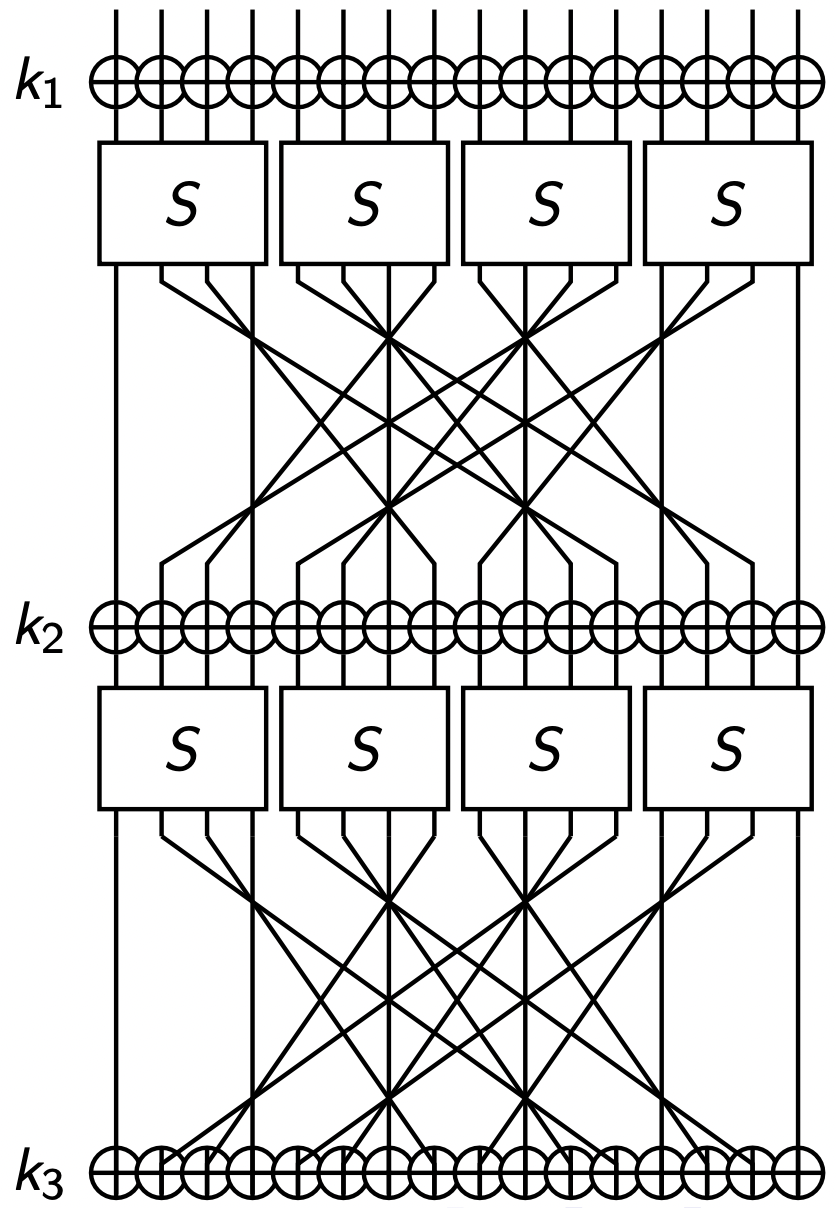
\includegraphics[width=\columnwidth]{SPN.png}\\
Repeat following for many rounds:
\begin{enumerate}
    \item Key mixing: Set $x=x\oplus k_i$
    \item Substitution: $x=S_1(x_1)||\cdots||S_8(x_8)$
    \item Permutation: Permute bits of $x$
\end{enumerate}

\end{multicols*}
\end{document}